\documentclass[a4paper,10pt]{article}
\usepackage{fullpage}
\usepackage{times}
\usepackage{hyperref}
\usepackage{graphicx}
\graphicspath{ {./images/} }

\begin{document}




\title{EDI: First Lab Report}
%Insert your name and ID inside the brackets
\author{Aiman Al Masoud - 502044}
\date{\today}

\maketitle

\begin{abstract}

Assignment 1: The goal of this work was to determine the average daily peak time of a server, using an active monitoring technique (traceroute).

\end{abstract}

\clearpage

\setcounter{page}{1}
%Figures and tables must be cited in the text and explained in detail.

\section{Monitoring of a Server's Peak Time}
%Insert a brief introduction of your first lab experience


\subsection{Methodology and experimental setup}


\maketitle
\subsubsection{Hypotheses that were formulated}


\underline{When a server is experiencing too many requests, the following things are expected to happen: }


\begin{itemize}

\item \label{hyp1} H1) Latency Surges: Because the server has to deal with a higher amount of packets per unit time, queueing is expected to happen, and the round trip time of packets sent to the server is expected to increase.

\item H2) Number of hops increases: At peak time, congestion may take place on the normally optimal routes, and thus alternative routes, which may include more hops, will be sought by the packets, increasing the average number of hops to reach the server.

\end{itemize}


\maketitle
\subsubsection{Experimental Setup}

A script that performs traceroute on a target IP at regular intervals (every 5 minutes) was executed on a vantage point for just over a week. Subsequently, the collected data was processed offline. 

The vantage point in question was a virtual machine on GCP (Google Cloud Platform), located on a server in the US. The target website was: www.google.it. Assuming that www.google.it is mostly visited by users in Italy, the timestamps were interpreted as times in CEST, aka: GMT+2, which happens to be the Italian local time in April.

As a side-note, peak time traditionally occurs from late evening to early night, more precisely from 6 PM to 11 PM. [\ref{article1}]

The assumption that I made, in accordance with H1[\ref{hyp1}], was that latency (RTT) would've been proportional to the amount of traffic on the server. 

\subsection{Experimental results}
%Present and discuss the experimental results that you have obtained

After letting the script run for more than 183 hours (almost 8 days), collecting measurements at regular intervals of 5 minutes, I was left with 2204 readings; 4 of which were discarded as outliers. 

The remaining 2200 measurements were processed and arranged in a table of this format:

\clearpage

\begin{table}[h!]
\centering
\begin{tabular}{|l|l|l|l|l|}
\hline
timestamp           & hops & reached & latency\_ms & hour \\ \hline
2022-04-17 16:09:56 & 15   & True    & 0.919000    & 16   \\ \hline
                    &      &         &             &      \\ \hline
                    &      &         &             &     
\end{tabular}
\caption{Table 1}
\label{fig:table1}
\end{table}


The records were grouped by hour of the day, the mean and standard error were computed, resulting in this final table:


\begin{table}[h!]
\centering

\begin{tabular}{|c|l|l|l|l|}
\hline
\multicolumn{1}{|l|}{hour} & latency\_ms & latency\_ms\_std\_err & hops      & hops\_std\_err \\ \hline
\textbf{0}                 & 0.885481    & 0.332606              & 12.326316 & 1.124600       \\ \hline
\textbf{1}                 & 0.911547    & 0.274709              & 12.784946 & 1.405343       \\ \hline
\textbf{2}                 & 0.923648    & 0.284790              & 12.562500 & 1.709494       \\ \hline
\textbf{3}                 & 0.883117    & 0.318890              & 12.436170 & 1.492335       \\ \hline
\textbf{4}                 & 0.951461    & 0.249570              & 12.702128 & 1.457865       \\ \hline
\textbf{5}                 & 0.915111    & 0.314960              & 12.252632 & 1.406432       \\ \hline
\textbf{6}                 & 0.955569    & 0.283697              & 12.138298 & 1.603766       \\ \hline
\textbf{7}                 & 0.914733    & 0.285439              & 12.357895 & 1.529259       \\ \hline
\textbf{8}                 & 0.876304    & 0.241643              & 12.463158 & 1.137471       \\ \hline
\textbf{9}                 & 0.909583    & 0.303091              & 12.361702 & 1.605441       \\ \hline
\textbf{10}                & 0.870383    & 0.259852              & 12.241758 & 1.628501       \\ \hline
\textbf{11}                & 0.877788    & 0.285976              & 12.559524 & 1.491754       \\ \hline
\textbf{12}                & 0.882918    & 0.348783              & 12.592593 & 1.376388       \\ \hline
\textbf{13}                & 0.897655    & 0.310639              & 12.180723 & 1.562866       \\ \hline
\textbf{14}                & 0.888898    & 0.280578              & 12.469880 & 1.417120       \\ \hline
\textbf{15}                & 0.827652    & 0.270974              & 12.271605 & 1.449244       \\ \hline
\textbf{16}                & 0.872984    & 0.279684              & 12.728261 & 1.597410       \\ \hline
\textbf{17}                & 0.846570    & 0.306079              & 12.505376 & 1.449315       \\ \hline
\textbf{18}                & 0.823714    & 0.301251              & 12.437500 & 1.159060       \\ \hline
\textbf{19}                & 0.870302    & 0.276282              & 12.800000 & 1.242852       \\ \hline
\textbf{20}                & 0.864380    & 0.286903              & 12.677419 & 1.286732       \\ \hline
\textbf{21}                & 0.892767    & 0.337298              & 12.505263 & 1.521993       \\ \hline
\textbf{22}                & 0.860239    & 0.356526              & 12.468085 & 1.300968       \\ \hline
\textbf{23}                & 0.933872    & 0.347573              & 12.606383 & 1.254824       \\ \hline
\end{tabular}

\caption{Table 2}
\label{fig:table2}

\end{table}


Two bar charts were obtained from said table.

\clearpage

\begin{figure}[h!]
\centering
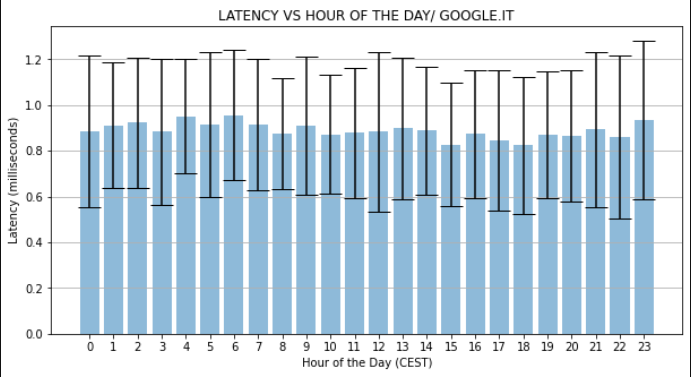
\includegraphics[scale=0.4]{latency_graph}
\caption{Latency Graph}
\label{fig:latency_graph}
\end{figure}

\begin{figure}[h!]
\centering
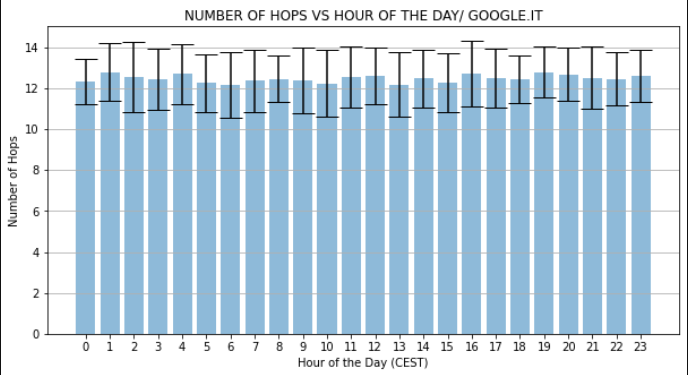
\includegraphics[scale=0.4]{hops_graph}
\caption{Hops Graph}
\label{fig:hops_graph}
\end{figure}




\section{Insert the title of your second lab}
%Insert a brief introduction of your second lab experience
\subsection{Methodology and experimental setup}
%Discuss your methodological approach and the plan/setup of your experiments
\subsection{Experimental results}
%Present and discuss the experimental results that you have obtained
\section{Conclusion}
%Insert couple of sentences that highlight the lessons you have learnt (if any) from these lab activities.


% idk, latex just needs this here for bibliography linking to work properly:
\clearpage

\section{References}


\begin{enumerate}

\item \label{article1}  \url{https://www.highspeedinternet.com/resources/why-does-my-internet-slow-down-at-night} 

\end{enumerate}







\end{document}